\documentclass[pdftex,12pt,a4paper]{article}

\input{/home/boris/science/tex_general/title_bor_utf8}


\newcommand{\doubledraw}[1]{
#1
\begin{minted}{tex}
#1
\end{minted}
}

\begin{document}
\parindent=0 pt % отступ равен 0

\tikzset{edge from parent/.style=
     {draw, edge from parent path={(\tikzparentnode) -- (\tikzchildnode)}}}


Реконструкция старого списка деревьев...


В идеале неплохо бы: слева дерево, справа его код.





\begin{enumerate}


\item 1
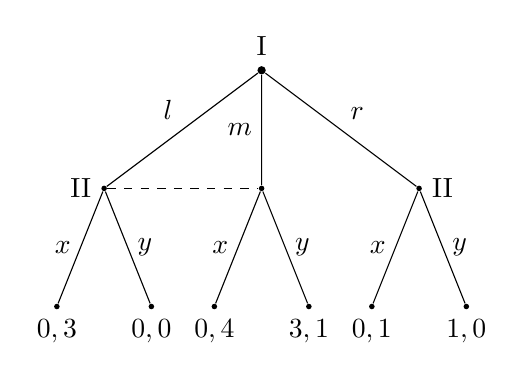
\begin{tikzpicture}[grow=down] % дерево
\tikzstyle{mystart} = [circle, minimum width=3pt,fill, inner sep=0pt] % starting node style
\tikzstyle{mydot} = [circle, minimum width=2pt,fill, inner sep=0pt] % decision node style
\tikzstyle{level 1}=[sibling distance=2cm] % расстояние между соседними узлами на одном уровне
\tikzstyle{level 2}=[sibling distance=1.2cm]
\tikzstyle{level 3}=[sibling distance=2cm]
\node[mystart, label=above: {I}] {} % создаем узел типа mydot, с пометкой "N" сверху и пустым текстом внутри узла
    child { node[mydot, label=left: {II}] (a) {}        
                	child {	node[mydot, label=below: {$0,3$}] {}
                	edge from parent node[left] {$x$}}
                	child {	node[mydot, label=below: {$0,0$}] {}
                	edge from parent node[right] {$y$}  }
    edge from parent node[above left] {$l$} }
    child { node[mydot] (b) {}        
                	child {	node[mydot, label=below: {$0,4$}] {}
                	edge from parent node[left] {$x$}}
                	child {	node[mydot, label=below: {$3,1$}] {}
                	edge from parent node[right] {$y$}  }
    edge from parent node[left] {$m$} }
    child { node[mydot, label=right: {II}] {}        
                	child {	node[mydot, label=below: {$0,1$}] {}
                	edge from parent node[left] {$x$}}
                	child {	node[mydot, label=below: {$1,0$}] {}
                	edge from parent node[right] {$y$}  }
    edge from parent node[above right] {$r$} } ;
\draw[dashed] (a)--(b);
\end{tikzpicture}

\item 2

\item 3

\item 4
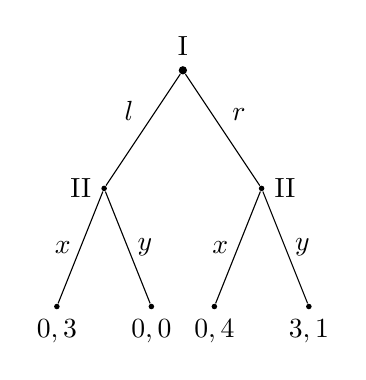
\begin{tikzpicture}[grow=down] % дерево
\tikzstyle{mystart} = [circle, minimum width=3pt,fill, inner sep=0pt] % starting node style
\tikzstyle{mydot} = [circle, minimum width=2pt,fill, inner sep=0pt] % decision node style
\tikzstyle{level 1}=[sibling distance=2cm] % расстояние между соседними узлами на одном уровне
\tikzstyle{level 2}=[sibling distance=1.2cm]
\tikzstyle{level 3}=[sibling distance=2cm]

\node[mystart, label=above: {I}] {} % создаем узел типа mydot, с пометкой "N" сверху и пустым текстом внутри узла
    child { node[mydot, label=left: {II}] (a) {}        
                	child {	node[mydot, label=below: {$0,3$}] {}
                	edge from parent node[left] {$x$}}
                	child {	node[mydot, label=below: {$0,0$}] {}
                	edge from parent node[right] {$y$}  }
    edge from parent node[above left] {$l$} }
    child { node[mydot, label=right: {II}] {}        
                	child {	node[mydot, label=below: {$0,4$}] {}
                	edge from parent node[left] {$x$}}
                	child {	node[mydot, label=below: {$3,1$}] {}
                	edge from parent node[right] {$y$}  }
    edge from parent node[above right] {$r$} } ;
\end{tikzpicture}

\item 5
\item 6
\item 7
\item 8
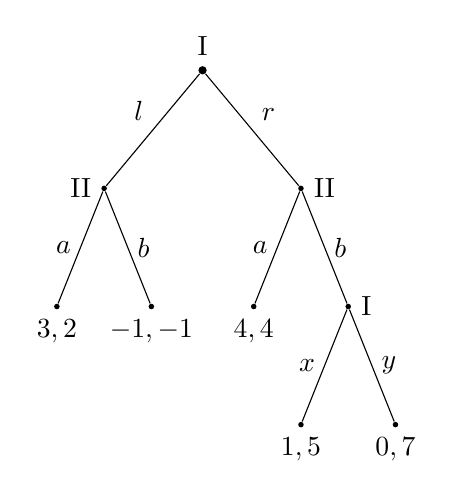
\begin{tikzpicture}[grow=down] % дерево
\tikzstyle{mystart} = [circle, minimum width=3pt,fill, inner sep=0pt] % starting node style
\tikzstyle{mydot} = [circle, minimum width=2pt,fill, inner sep=0pt] % decision node style
\tikzstyle{level 1}=[sibling distance=2.5cm] % расстояние между соседними узлами на одном уровне
\tikzstyle{level 2}=[sibling distance=1.2cm]
\tikzstyle{level 3}=[sibling distance=1.2cm]

\node[mystart, label=above: {I}] {} % создаем узел типа mydot, с пометкой "N" сверху и пустым текстом внутри узла
    child { node[mydot, label=left: {II}] (a) {}        
                	child {	node[mydot, label=below: {$3,2$}] {}
                	edge from parent node[left] {$a$}}
                	child {	node[mydot, label=below: {$-1,-1$}] {}
                	edge from parent node[right] {$b$}  }
    edge from parent node[above left] {$l$} }
    child { node[mydot, label=right: {II}] {}        
                	child {	node[mydot, label=below: {$4,4$}] {}
                	edge from parent node[left] {$a$}}
                	child {	node[mydot, label=right: {I}] {}
                    child { node[mydot, label=below: {$1,5$}] {}
                    edge from parent node[left] {$x$} }
                    child { node[mydot, label=below: {$0,7$}] {}
                    edge from parent node[right] {$y$} }                	
               	edge from parent node[right] {$b$}  }
    edge from parent node[above right] {$r$} } ;
\end{tikzpicture}

\item 9
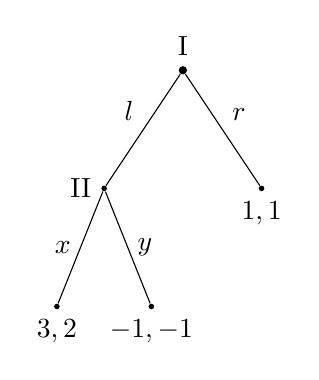
\begin{tikzpicture}[grow=down] % дерево
\tikzstyle{mystart} = [circle, minimum width=3pt,fill, inner sep=0pt] % starting node style
\tikzstyle{mydot} = [circle, minimum width=2pt,fill, inner sep=0pt] % decision node style
\tikzstyle{level 1}=[sibling distance=2cm] % расстояние между соседними узлами на одном уровне
\tikzstyle{level 2}=[sibling distance=1.2cm]
\tikzstyle{level 3}=[sibling distance=2cm]

\node[mystart, label=above: {I}] {} % создаем узел типа mydot, с пометкой "N" сверху и пустым текстом внутри узла
    child { node[mydot, label=left: {II}] (a) {}        
                	child {	node[mydot, label=below: {$3,2$}] {}
                	edge from parent node[left] {$x$}}
                	child {	node[mydot, label=below: {$-1,-1$}] {}
                	edge from parent node[right] {$y$}  }
    edge from parent node[above left] {$l$} } 
    child { node[mydot, label=below: {$1,1$}] {}        
    edge from parent node[above right] {$r$} } ;
\end{tikzpicture}

\item 10
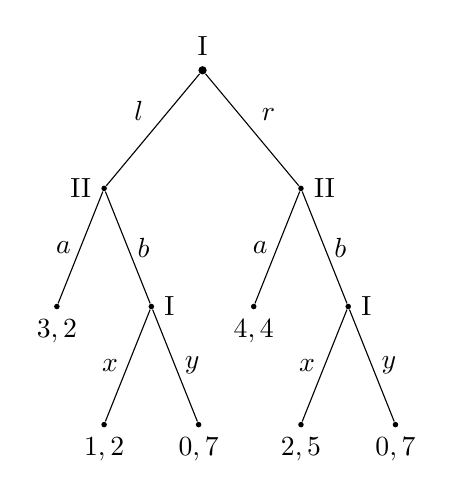
\begin{tikzpicture}[grow=down] % дерево
\tikzstyle{mystart} = [circle, minimum width=3pt,fill, inner sep=0pt] % starting node style
\tikzstyle{mydot} = [circle, minimum width=2pt,fill, inner sep=0pt] % decision node style
\tikzstyle{level 1}=[sibling distance=2.5cm] % расстояние между соседними узлами на одном уровне
\tikzstyle{level 2}=[sibling distance=1.2cm]
\tikzstyle{level 3}=[sibling distance=1.2cm]

\node[mystart, label=above: {I}] {} % создаем узел типа mydot, с пометкой "N" сверху и пустым текстом внутри узла
    child { node[mydot, label=left: {II}] (a) {}        
                	child {	node[mydot, label=below: {$3,2$}] {}
                	edge from parent node[left] {$a$}}
                	child {	node[mydot, label=right: {I}] {}
                    child { node[mydot, label=below: {$1,2$}] {}
                    edge from parent node[left] {$x$} }
                    child { node[mydot, label=below: {$0,7$}] {}
                    edge from parent node[right] {$y$} }                	
                	edge from parent node[right] {$b$}  }
    edge from parent node[above left] {$l$} }
    child { node[mydot, label=right: {II}] {}        
                	child {	node[mydot, label=below: {$4,4$}] {}
                	edge from parent node[left] {$a$}}
                	child {	node[mydot, label=right: {I}] {}
                    child { node[mydot, label=below: {$2,5$}] {}
                    edge from parent node[left] {$x$} }
                    child { node[mydot, label=below: {$0,7$}] {}
                    edge from parent node[right] {$y$} }                	
               	edge from parent node[right] {$b$}  }
    edge from parent node[above right] {$r$} } ;
\end{tikzpicture}


\item 11
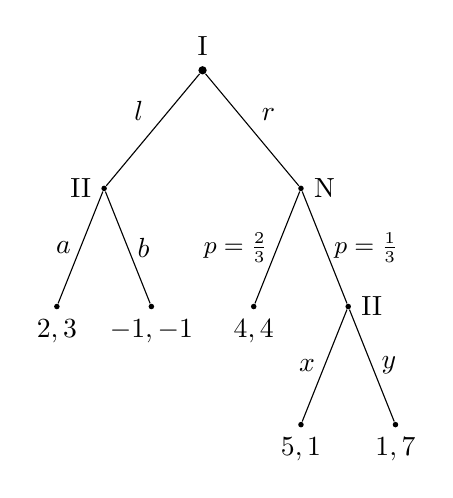
\begin{tikzpicture}[grow=down] % дерево
\tikzstyle{mystart} = [circle, minimum width=3pt,fill, inner sep=0pt] % starting node style
\tikzstyle{mydot} = [circle, minimum width=2pt,fill, inner sep=0pt] % decision node style
\tikzstyle{level 1}=[sibling distance=2.5cm] % расстояние между соседними узлами на одном уровне
\tikzstyle{level 2}=[sibling distance=1.2cm]
\tikzstyle{level 3}=[sibling distance=1.2cm]

\node[mystart, label=above: {I}] {} % создаем узел типа mydot, с пометкой "N" сверху и пустым текстом внутри узла
    child { node[mydot, label=left: {II}] (a) {}        
                	child {	node[mydot, label=below: {$2,3$}] {}
                	edge from parent node[left] {$a$}}
                	child {	node[mydot, label=below: {$-1,-1$}] {}
                	edge from parent node[right] {$b$}  }
    edge from parent node[above left] {$l$} }
    child { node[mydot, label=right: {N}] {}        
                	child {	node[mydot, label=below: {$4,4$}] {}
                	edge from parent node[left] {{\small $p=\frac{2}{3}$}}}
                	child {	node[mydot, label=right: {II}] {}
                    child { node[mydot, label=below: {$5,1$}] {}
                    edge from parent node[left] {$x$} }
                    child { node[mydot, label=below: {$1,7$}] {}
                    edge from parent node[right] {$y$} }                	
               	edge from parent node[right] {{\small $p=\frac{1}{3}$}}  }
    edge from parent node[above right] {$r$} } ;
\end{tikzpicture}

\item 12
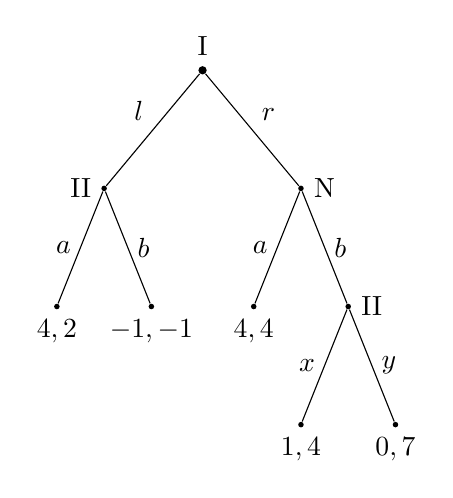
\begin{tikzpicture}[grow=down] % дерево
\tikzstyle{mystart} = [circle, minimum width=3pt,fill, inner sep=0pt] % starting node style
\tikzstyle{mydot} = [circle, minimum width=2pt,fill, inner sep=0pt] % decision node style
\tikzstyle{level 1}=[sibling distance=2.5cm] % расстояние между соседними узлами на одном уровне
\tikzstyle{level 2}=[sibling distance=1.2cm]
\tikzstyle{level 3}=[sibling distance=1.2cm]

\node[mystart, label=above: {I}] {} % создаем узел типа mydot, с пометкой "N" сверху и пустым текстом внутри узла
    child { node[mydot, label=left: {II}] (a) {}        
                	child {	node[mydot, label=below: {$4,2$}] {}
                	edge from parent node[left] {$a$}}
                	child {	node[mydot, label=below: {$-1,-1$}] {}
                	edge from parent node[right] {$b$}  }
    edge from parent node[above left] {$l$} }
    child { node[mydot, label=right: {N}] {}        
                	child {	node[mydot, label=below: {$4,4$}] {}
                	edge from parent node[left] {$a$}}
                	child {	node[mydot, label=right: {II}] {}
                    child { node[mydot, label=below: {$1,4$}] {}
                    edge from parent node[left] {$x$} }
                    child { node[mydot, label=below: {$0,7$}] {}
                    edge from parent node[right] {$y$} }                	
               	edge from parent node[right] {$b$}  }
    edge from parent node[above right] {$r$} } ;
\end{tikzpicture}


\item 13
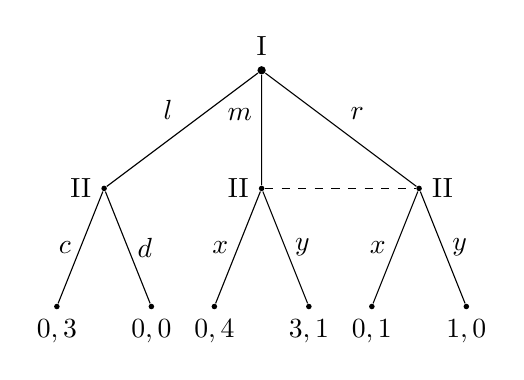
\begin{tikzpicture}[grow=down] % дерево
\tikzstyle{mystart} = [circle, minimum width=3pt,fill, inner sep=0pt] % starting node style
\tikzstyle{mydot} = [circle, minimum width=2pt,fill, inner sep=0pt] % decision node style
\tikzstyle{level 1}=[sibling distance=2cm] % расстояние между соседними узлами на одном уровне
\tikzstyle{level 2}=[sibling distance=1.2cm]
\tikzstyle{level 3}=[sibling distance=2cm]

\node[mystart, label=above: {I}] {} % создаем узел типа mydot, с пометкой "N" сверху и пустым текстом внутри узла
    child { node[mydot, label=left: {II}] {}        
                	child {	node[mydot, label=below: {$0,3$}] {}
                	edge from parent node[left] {$c$}}
                	child {	node[mydot, label=below: {$0,0$}] {}
                	edge from parent node[right] {$d$}  }
    edge from parent node[above left] {$l$} }
    child { node[mydot, label=left: {II}] (a) {}        
                	child {	node[mydot, label=below: {$0,4$}] {}
                	edge from parent node[left] {$x$}}
                	child {	node[mydot, label=below: {$3,1$}] {}
                	edge from parent node[right] {$y$}  }
    edge from parent node[above left] {$m$} }
    child { node[mydot, label=right: {II}] (b) {}        
                	child {	node[mydot, label=below: {$0,1$}] {}
                	edge from parent node[left] {$x$}}
                	child {	node[mydot, label=below: {$1,0$}] {}
                	edge from parent node[right] {$y$}  }
    edge from parent node[above right] {$r$} } ;
\draw[dashed] (a)--(b);
\end{tikzpicture}


\item 14
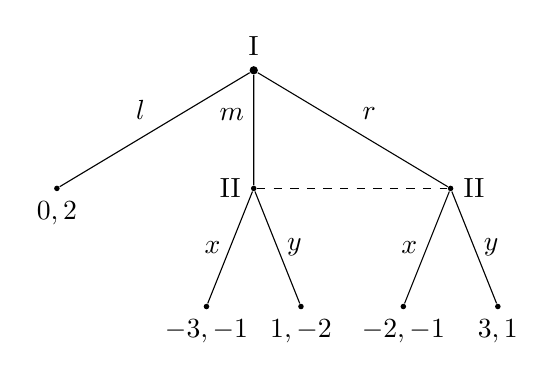
\begin{tikzpicture}[grow=down] % дерево
\tikzstyle{mystart} = [circle, minimum width=3pt,fill, inner sep=0pt] % starting node style
\tikzstyle{mydot} = [circle, minimum width=2pt,fill, inner sep=0pt] % decision node style
\tikzstyle{level 1}=[sibling distance=2.5cm] % расстояние между соседними узлами на одном уровне
\tikzstyle{level 2}=[sibling distance=1.2cm]
\tikzstyle{level 3}=[sibling distance=2cm]

\node[mystart, label=above: {I}] {} % создаем узел типа mydot, с пометкой "N" сверху и пустым текстом внутри узла
    child { node[mydot, label=below: {$0,2$}] {}        
    edge from parent node[above left] {$l$} }
    child { node[mydot, label=left: {II}] (a) {}        
                	child {	node[mydot, label=below: {$-3,-1$}] {}
                	edge from parent node[left] {$x$}}
                	child {	node[mydot, label=below: {$1,-2$}] {}
                	edge from parent node[right] {$y$}  }
    edge from parent node[above left] {$m$} }
    child { node[mydot, label=right: {II}] (b) {}        
                	child {	node[mydot, label=below: {$-2,-1$}] {}
                	edge from parent node[left] {$x$}}
                	child {	node[mydot, label=below: {$3,1$}] {}
                	edge from parent node[right] {$y$}  }
    edge from parent node[above right] {$r$} } ;
\draw[dashed] (a)--(b);
\end{tikzpicture}


\item 15
\begin{tikzpicture}[grow=down] % дерево
\tikzstyle{mystart} = [circle, minimum width=3pt,fill, inner sep=0pt] % starting node style
\tikzstyle{mydot} = [circle, minimum width=2pt,fill, inner sep=0pt] % decision node style
\tikzstyle{level 1}=[sibling distance=2cm] % расстояние между соседними узлами на одном уровне
\tikzstyle{level 2}=[sibling distance=2cm]
\tikzstyle{level 3}=[sibling distance=2cm]
\node[mystart, label=above: {I}] {} % создаем узел типа mydot, с пометкой "N" сверху и пустым текстом внутри узла
    child { node[mydot, label=below: {$-1,1$}] {}        
    edge from parent node[left] {$l$} }
    child { node[mydot, label=above: {II} ] {}        
        child { node[mydot, label=below: {$4,4$}] {} 
        edge from parent node[left] {$c$} }
        child { node[mydot, label=above: {I}] (b) {}
                	child {	node[mydot, label=below: {$1,5$}] {}
                	edge from parent node[left] {$x$}}
                	child {	node[mydot, label=below: {$0,7$}] {}
                	edge from parent node[right] {$y$}  }
        edge from parent node[right] {$d$} }
    edge from parent node[right] {$r$} };
\end{tikzpicture}

\item 16
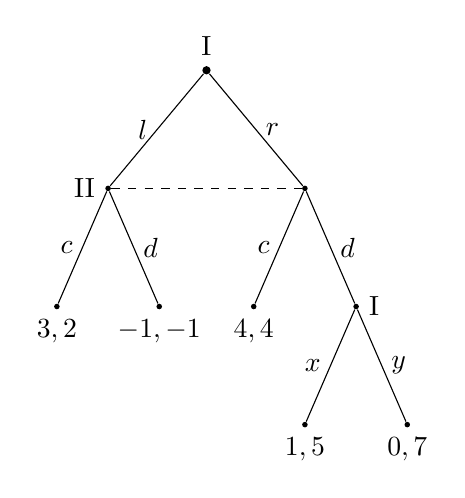
\begin{tikzpicture}[grow=down] % дерево
\tikzstyle{mystart} = [circle, minimum width=3pt,fill, inner sep=0pt] % starting node style
\tikzstyle{mydot} = [circle, minimum width=2pt,fill, inner sep=0pt] % decision node style
\tikzstyle{level 1}=[sibling distance=2.5cm] % расстояние между соседними узлами на одном уровне
\tikzstyle{level 2}=[sibling distance=1.3cm]
\tikzstyle{level 3}=[sibling distance=1.3cm]
\node[mystart, label=above: {I}] {} % создаем узел типа mydot, с пометкой "N" сверху и пустым текстом внутри узла
    child { node[mydot, label=left: {II}] (a) {}        
        child { node[mydot, label=below: {$3,2$}] {} 
        edge from parent node[left] {$c$} }
        child { node[mydot, label=below: {$-1,-1$}] (b) {}
        edge from parent node[right] {$d$} }
    edge from parent node[left] {$l$} }
    child { node[mydot ] (b) {}        
        child { node[mydot, label=below: {$4,4$}] {} 
        edge from parent node[left] {$c$} }
        child { node[mydot, label=right: {I}] {}
                	child {	node[mydot, label=below: {$1,5$}] {}
                	edge from parent node[left] {$x$}}
                	child {	node[mydot, label=below: {$0,7$}] {}
                	edge from parent node[right] {$y$}  }
        edge from parent node[right] {$d$} }
    edge from parent node[right] {$r$} };
\draw[dashed] (a)--(b);
\end{tikzpicture}


\item Дерево
\begin{tikzpicture}[grow=down] % дерево
\tikzstyle{mystart} = [circle, minimum width=3pt,fill, inner sep=0pt] % starting node style
\tikzstyle{mydot} = [circle, minimum width=2pt,fill, inner sep=0pt] % decision node style
\tikzstyle{level 1}=[sibling distance=4cm] % расстояние между соседними узлами на одном уровне
\tikzstyle{level 2}=[sibling distance=2cm]
\tikzstyle{level 3}=[sibling distance=2cm]
\node[mystart, label=above: {I}] {} % создаем узел типа mydot, с пометкой "N" сверху и пустым текстом внутри узла
    child { node[mydot, label=above: {II}] {}
    	child { node[mydot, label=below: {$3,2$}] {} 
		edge from parent node[left] {$a$} }        
    	child {	node[mydot, label=below: {$-1,-1$}] {} 
		edge from parent node[right] {$b$} } 
    edge from parent node[left] {$l$} }
    child { node[mydot, label=above: {II} ] {}        
        child { node[mydot, label=below: {$4,4$}] {} 
        edge from parent node[left] {$c$} }
        child { node[mydot, label=above: {I}] (b) {}
        	child { node[mydot, label=below: {$1,5$}] {}
            edge from parent node[left] {$x$}}
            child {	node[mydot, label=below: {$0,7$}] {}
            edge from parent node[right] {$y$}  }
        edge from parent node[right] {$d$} }
    edge from parent node[right] {$r$} };
\end{tikzpicture}

\item Дерево
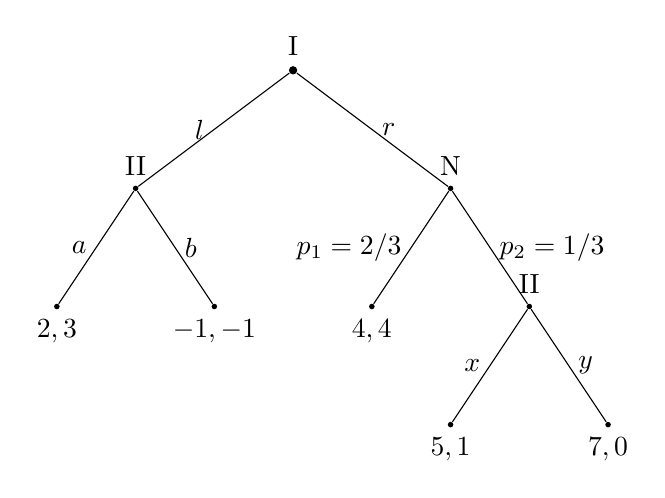
\begin{tikzpicture}[grow=down] % дерево
\tikzstyle{mystart} = [circle, minimum width=3pt,fill, inner sep=0pt] % starting node style
\tikzstyle{mydot} = [circle, minimum width=2pt,fill, inner sep=0pt] % decision node style
\tikzstyle{level 1}=[sibling distance=4cm] % расстояние между соседними узлами на одном уровне
\tikzstyle{level 2}=[sibling distance=2cm]
\tikzstyle{level 3}=[sibling distance=2cm]
\node[mystart, label=above: {I}] {} % создаем узел типа mydot, с пометкой "N" сверху и пустым текстом внутри узла
    child { node[mydot, label=above: {II}] {}
    	child { node[mydot, label=below: {$2,3$}] {} 
		edge from parent node[left] {$a$} }        
    	child {	node[mydot, label=below: {$-1,-1$}] {} 
		edge from parent node[right] {$b$} } 
    edge from parent node[left] {$l$} }
    child { node[mydot, label=above: {N} ] {}        
        child { node[mydot, label=below: {$4,4$}] {} 
        edge from parent node[left] {$p_1=2/3$} }
        child { node[mydot, label=above: {II}] (b) {}
                child { node[mydot, label=below: {$5,1$}] {}
              	edge from parent node[left] {$x$}}
                child { node[mydot, label=below: {$7,0$}] {}
               	edge from parent node[right] {$y$}  }
        edge from parent node[right] {$p_2=1/3$} }
    edge from parent node[right] {$r$} };
\end{tikzpicture}







\item 
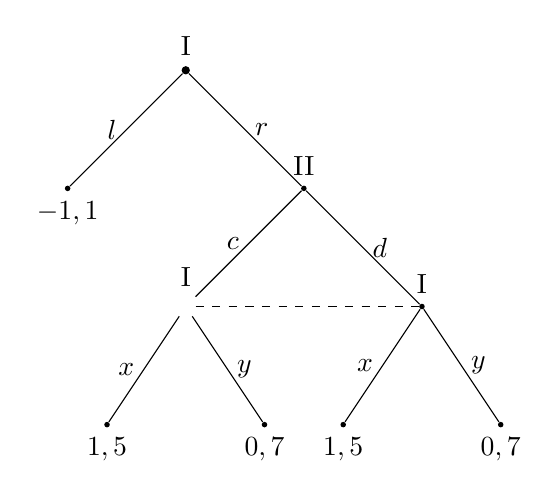
\begin{tikzpicture}[grow=down] % дерево
\tikzstyle{mystart} = [circle, minimum width=3pt,fill, inner sep=0pt] % starting node style
\tikzstyle{mydot} = [circle, minimum width=2pt,fill, inner sep=0pt] % decision node style
\tikzstyle{level 1}=[sibling distance=3cm] % расстояние между соседними узлами на одном уровне
\tikzstyle{level 2}=[sibling distance=3cm]
\tikzstyle{level 3}=[sibling distance=2cm]
\node[mystart, label=above: {I}] {} % создаем узел типа mydot, с пометкой "I" сверху и пустым текстом внутри узла
    child { node[mydot, label=below: {$-1,1$}] {}        
    edge from parent node[left] {$l$} }
    child { node[mydot, label=above: {II} ] {}        
        child { node[label=above: {I}] (a) {} 
                child { node[mydot, label=below: {$1,5$}] {}
               	edge from parent node[left] {$x$}}
                child { node[mydot, label=below: {$0,7$}] {}
               	edge from parent node[right] {$y$}  }
        edge from parent node[left] {$c$} }
        child { node[mydot, label=above: {I}] (b) {}
                child {	node[mydot, label=below: {$1,5$}] {}
              	edge from parent node[left] {$x$}}
                child { node[mydot, label=below: {$0,7$}] {}
               	edge from parent node[right] {$y$}  }
        edge from parent node[right] {$d$} }
    edge from parent node[right] {$r$} };
\draw[dashed] (a)--(b);
\end{tikzpicture}



\item

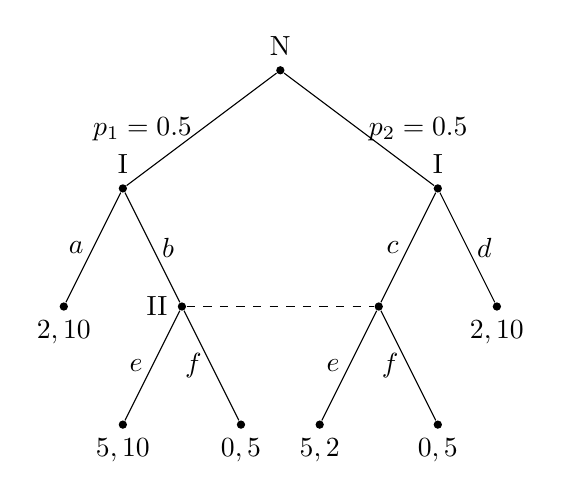
\begin{tikzpicture}[grow=down] % дерево
\tikzstyle{mydot} = [circle, minimum width=3pt,fill, inner sep=0pt] % размеры точки в центре узла
\tikzstyle{level 1}=[sibling distance=4cm] % расстояние между соседними узлами на одном уровне
\tikzstyle{level 2}=[sibling distance=1.5cm]
\tikzstyle{level 3}=[sibling distance=1.5cm]

\node[mydot, label=above: {N}] {}
	child { node[mydot, label=above: {I}] {}
			child { node[mydot, label=below: {$2,10$}] {}
     		edge from parent node[left] {$a$} }
			child { node[mydot, label=left: {II} ] (a) {}
					child { node[mydot, label=below: {$5,10$}] {}
					edge from parent node[left] {$e$} }
					child { node[mydot, label=below: {$0,5$}] {}
					edge from parent node[left] {$f$} }
	    	edge from parent node[right] {$b$} }
	edge from parent node[left] {$p_1=0.5$} }
	child { node[mydot, label=above: {I}] {}
			child { node[mydot] (b) {}
					child {	node[mydot, label=below: {$5,2$}] {}
					edge from parent node[left] {$e$} }
  					child {	node[mydot, label=below: {$0,5$}] {}
					edge from parent node[left] {$f$} }
			edge from parent node[left] {$c$} }
			child {	node[mydot, label=below: {$2,10$}] {}
			edge from parent node[right] {$d$} }
	edge from parent node[right] {$p_2=0.5$} } ;
\draw[dashed] (a)--(b);
\end{tikzpicture}



\item 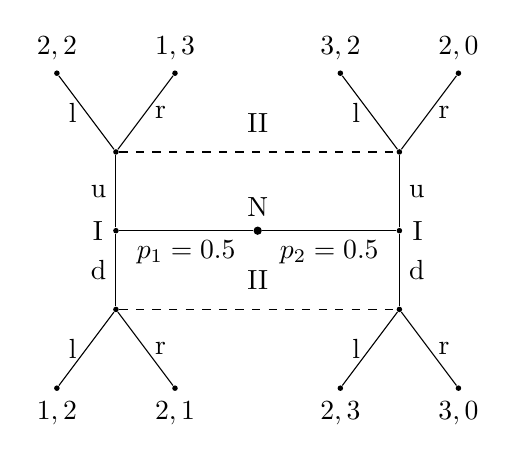
\begin{tikzpicture} % Паук
\tikzstyle{mydot} = [circle, minimum width=2pt,fill, inner sep=0pt] % decision node style
\tikzstyle{mystart} = [circle, minimum width=3pt,fill, inner sep=0pt] % strating node style
\tikzstyle{level 1}=[sibling distance=2cm] % расстояние между соседними узлами на одном уровне
\tikzstyle{level 1}=[level distance=1.8cm] % длина веточки на первом уровне
\tikzstyle{level 2}=[sibling distance=2cm]
\tikzstyle{level 2}=[level distance=1cm]
\tikzstyle{level 3}=[sibling distance=2cm]
\tikzstyle{level 3}=[level distance=1cm]

%
\node[mystart, label=above: {N}] {}
	child[grow=left] {node[mydot, label=left: {I}] {} % left side of the spider
		child[grow=up] {node[mydot] (U1) {} [grow=up]
			child {node[mydot, label=above: {$1,3$}] {}
			edge from parent node[right] {r} }
			child {node[mydot, label=above: {$2,2$}] {}
			edge from parent node[left] {l} }
		edge from parent node[left] {u} }
		child[grow=down] {node[mydot] (D1) {} [grow=down]
			child {node[mydot, label=below: {$1,2$}] {}
			edge from parent node[left] {l} }
			child {node[mydot, label=below: {$2,1$}] {}
			edge from parent node[right] {r} }
		edge from parent node[left] {d} }
    edge from parent node[below] {$p_1=0.5$} }
%
	child[grow=right] {node[mydot, label=right: {I}] {} % right side of the spider
		child[grow=up] {node[mydot] (U2) {} [grow=up]
			child {node[mydot, label=above: {$2,0$}] {}
			edge from parent node[right] {r} }
			child {node[mydot, label=above: {$3,2$}] {}
			edge from parent node[left] {l} }
		edge from parent node[right] {u} }
		child[grow=down] {node[mydot] (D2) {} [grow=down]
			child {node[mydot, label=below: {$2,3$}] {}
			edge from parent node[left] {l} }
			child {node[mydot, label=below: {$3,0$}] {}
			edge from parent node[right] {r} }
		edge from parent node[right] {d} }
    edge from parent node[below] {$p_2=0.5$} } ;
\draw[dashed] (U1)--node[label=above:II] {}(U2);
\draw[dashed] (D1)--node[label=above:II] {}(D2);
\end{tikzpicture}



\item
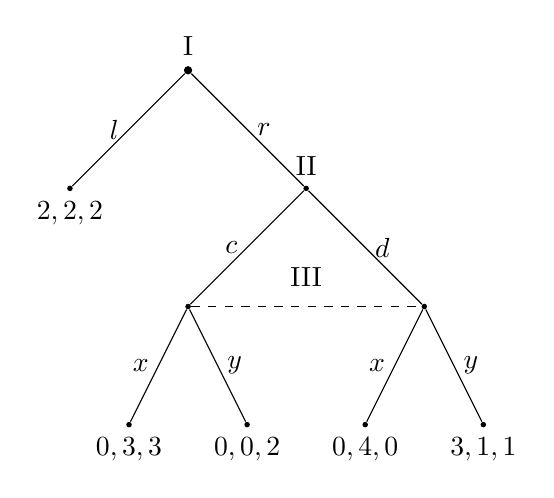
\begin{tikzpicture} % три игрока с выходом первого
\tikzstyle{mydot} = [circle, minimum width=2pt,fill, inner sep=0pt] % decision node style
\tikzstyle{mystart} = [circle, minimum width=3pt,fill, inner sep=0pt] % strating node style
\tikzstyle{level 1}=[level distance=1.5cm] % длина линии
\tikzstyle{level 2}=[level distance=1.5cm] % длина линии
\tikzstyle{level 3}=[level distance=1.5cm] % длина линии
\tikzstyle{level 1}=[sibling distance=3cm] % расстояние между соседними узлами на одном уровне
\tikzstyle{level 2}=[sibling distance=3cm]
\tikzstyle{level 3}=[sibling distance=1.5cm]
\node[mystart, label=above: {I}] {} % создаем узел типа mydot, с пометкой "I" сверху и пустым текстом внутри узла
    child { node[mydot, label=below: {$2,2,2$}] {}        
    edge from parent node[left] {$l$} }
    child { node[mydot, label=above: {II} ] {}        
        child { node[mydot] (a) {} 
                	child {	node[mydot, label=below: {$0,3,3$}] {}
                	edge from parent node[left] {$x$}}
                	child {	node[mydot, label=below: {$0,0,2$}] {}
                	edge from parent node[right] {$y$}  }
        edge from parent node[left] {$c$} }
        child { node[mydot] (b) {}
                	child {	node[mydot, label=below: {$0,4,0$}] {}
                	edge from parent node[left] {$x$}}
                	child {	node[mydot, label=below: {$3,1,1$}] {}
                	edge from parent node[right] {$y$}  }
        edge from parent node[right] {$d$} }
    edge from parent node[right] {$r$} };
\draw[dashed] (a)--node[label=above: {III}] {}(b);
\end{tikzpicture}



\item


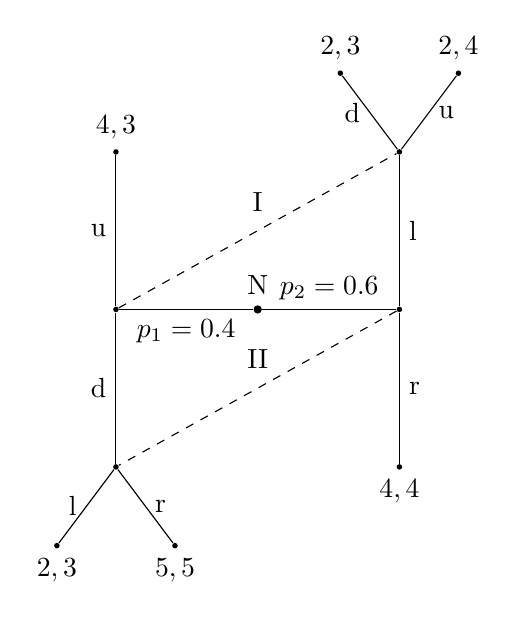
\begin{tikzpicture} % укороченный паук
\tikzstyle{mydot} = [circle, minimum width=2pt,fill, inner sep=0pt] % decision node style
\tikzstyle{mystart} = [circle, minimum width=3pt,fill, inner sep=0pt] % strating node style
\tikzstyle{level 1}=[sibling distance=2cm] % расстояние между соседними узлами на одном уровне
\tikzstyle{level 1}=[level distance=1.8cm] % длина веточки на первом уровне
\tikzstyle{level 2}=[sibling distance=2cm]
\tikzstyle{level 2}=[level distance=2cm]
\tikzstyle{level 3}=[sibling distance=2cm]
\tikzstyle{level 3}=[level distance=1cm]

%
\node[mystart, label=above: {N}] {}
	child[grow=left] {node[mydot] (ia) {} % left side of the spider
		child[grow=up] {node[mydot,label=above: {$4,3$}] {} [grow=up] 
		edge from parent node[left] {u} }
		child[grow=down] {node[mydot] (iib) {} [grow=down]
			child {node[mydot, label=below: {$2,3$}] {}
			edge from parent node[left] {l} }
			child {node[mydot, label=below: {$5,5$}] {}
			edge from parent node[right] {r} }
		edge from parent node[left] {d} }
    edge from parent node[below] {$p_1=0.4$} }
%
	child[grow=right] {node[mydot] (iia) {} % right side of the spider
		child[grow=up] {node[mydot] (ib) {} [grow=up]
			child {node[mydot, label=above: {$2,4$}] {}
			edge from parent node[right] {u} }
			child {node[mydot, label=above: {$2,3$}] {}
			edge from parent node[left] {d} }
		edge from parent node[right] {l} }
		child[grow=down] {node[mydot,label=below: {$4,4$}] {} [grow=down] 
		edge from parent node[right] {r} }
    edge from parent node[above] {$p_2=0.6$} } ;
\draw[dashed] (ia)--node[label=above:I] {}(ib);
\draw[dashed] (iia)--node[label=above:II] {}(iib);
\end{tikzpicture}



\item 
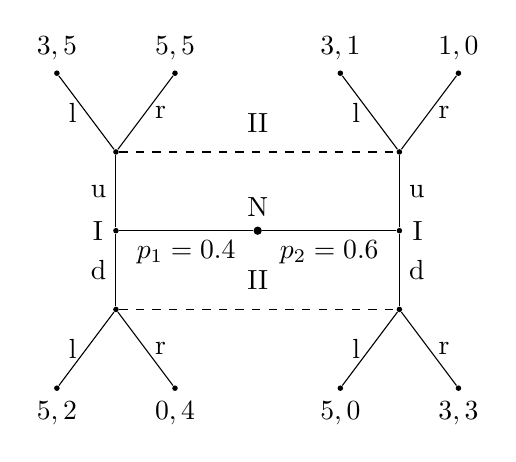
\begin{tikzpicture} % Паук
\tikzstyle{mydot} = [circle, minimum width=2pt,fill, inner sep=0pt] % decision node style
\tikzstyle{mystart} = [circle, minimum width=3pt,fill, inner sep=0pt] % strating node style
\tikzstyle{level 1}=[sibling distance=2cm] % расстояние между соседними узлами на одном уровне
\tikzstyle{level 1}=[level distance=1.8cm] % длина веточки на первом уровне
\tikzstyle{level 2}=[sibling distance=2cm]
\tikzstyle{level 2}=[level distance=1cm]
\tikzstyle{level 3}=[sibling distance=2cm]
\tikzstyle{level 3}=[level distance=1cm]

%
\node[mystart, label=above: {N}] {}
	child[grow=left] {node[mydot, label=left: {I}] {} % left side of the spider
		child[grow=up] {node[mydot] (U1) {} [grow=up]
			child {node[mydot, label=above: {$5,5$}] {}
			edge from parent node[right] {r} }
			child {node[mydot, label=above: {$3,5$}] {}
			edge from parent node[left] {l} }
		edge from parent node[left] {u} }
		child[grow=down] {node[mydot] (D1) {} [grow=down]
			child {node[mydot, label=below: {$5,2$}] {}
			edge from parent node[left] {l} }
			child {node[mydot, label=below: {$0,4$}] {}
			edge from parent node[right] {r} }
		edge from parent node[left] {d} }
    edge from parent node[below] {$p_1=0.4$} }
%
	child[grow=right] {node[mydot, label=right: {I}] {} % right side of the spider
		child[grow=up] {node[mydot] (U2) {} [grow=up]
			child {node[mydot, label=above: {$1,0$}] {}
			edge from parent node[right] {r} }
			child {node[mydot, label=above: {$3,1$}] {}
			edge from parent node[left] {l} }
		edge from parent node[right] {u} }
		child[grow=down] {node[mydot] (D2) {} [grow=down]
			child {node[mydot, label=below: {$5,0$}] {}
			edge from parent node[left] {l} }
			child {node[mydot, label=below: {$3,3$}] {}
			edge from parent node[right] {r} }
		edge from parent node[right] {d} }
    edge from parent node[below] {$p_2=0.6$} } ;
\draw[dashed] (U1)--node[label=above:II] {}(U2);
\draw[dashed] (D1)--node[label=above:II] {}(D2);
\end{tikzpicture}




\end{enumerate}
\end{document}